\documentclass[11pt]{article}
\usepackage{latexsym}
\usepackage{amsmath}
\usepackage{amssymb}
\usepackage{amsthm}
\usepackage{epsfig}
\usepackage{bbm}
\usepackage[tight]{subfigure}

\usepackage{amsmath}

\DeclareMathOperator*{\minimize}{min}
\DeclareMathOperator*{\maximize}{max}

\usepackage{algorithm}
 %on linux you may need to run sudo apt-get install texlive-full to install algorithm.sys
% \usepackage{algorithmic}
\usepackage{algpseudocode}

\usepackage{verbatim}

\newcommand{\handout}[5]{
  \noindent
  \begin{center}
  \framebox{
    \vbox{
      \hbox to 5.78in { {#1} \hfill #2 }
      \vspace{4mm}
      \hbox to 5.78in { {\Large \hfill #5  \hfill} }
      \vspace{2mm}
      \hbox to 5.78in { {\em #3 \hfill #4} }
    }
  }
  \end{center}
  \vspace*{4mm}
}

\newcommand{\lecture}[5]{\handout{#1}{#2}{#3}{#4}{#5}}
\newcommand{\collision}[0]{\mathrm{collision}}
\newcommand{\nocollision}[0]{\overline{\collision}}

\newcommand*{\QED}{\hfill\ensuremath{\square}}

\newtheorem{theorem}{Theorem}
\newtheorem{corollary}[theorem]{Corollary}
\newtheorem{lemma}[theorem]{Lemma}
\newtheorem{observation}[theorem]{Observation}
\newtheorem{proposition}[theorem]{Proposition}
\newtheorem{definition}[theorem]{Definition}
\newtheorem{claim}[theorem]{Claim}
\newtheorem{fact}[theorem]{Fact}
\newtheorem{assumption}[theorem]{Assumption}
\newtheorem{note}[theorem]{Note}

% 1-inch margins, from fullpage.sty by H.Partl, Version 2, Dec. 15, 1988.
\topmargin 0pt
\advance \topmargin by -\headheight
\advance \topmargin by -\headsep
\textheight 8.9in
\oddsidemargin 0pt
\evensidemargin \oddsidemargin
\marginparwidth 0.5in
\textwidth 6.5in

\parindent 0in
\parskip 1.5ex
%\renewcommand{\baselinestretch}{1.25}

\begin{document}

\lecture{Statistical Techniques in Robotics (16-831, S21)}{Lecture \#24
  (Wednesday, May 5)}{Lecturer: Kris Kitani}{Scribes: Samuel Triest, Ingrid Navarro}{ MaxEnt IRL and GAIL}

\section{Review}

This section briefly surveys the topics covered during the previous lecture. These include: Matrix Game IRL, Maximum Margin IRL, and Maximum Margin Planning.

\subsection{Matrix Game IRL}

In the previous lecture we derived a game theoretic approach to the IRL problem following \cite{MGIRL}. In this paradigm, we used the policy value shown below to derive our objective:
\begin{equation}
    V(\pi) = \theta \cdot \mu(\pi),
\end{equation}

We discussed that the Matrix Game IRL wants to find the value of the expert's policy $\pi_E$ that is better than any other policy, i.e.,
\begin{align}
    V(\pi_E) &\geq V(\pi) \\
    \theta \cdot \mu(\pi_E) &\geq \theta \cdot \mu(\pi)
\end{align}

In fact, we want to have the largest possible difference between these two terms. We, thus, wrote this objective function as a minimum over the whole function with a maximum expected value of the next best policy
\begin{equation}
    \minimize_{\theta}\{\maximize_{\pi} \theta \cdot \mu(\pi) - \theta \cdot \mu(\pi_E)\}.
\end{equation}

By further re-arranging the terms of this objective, we revealed the notation of the two-player game \eqref{eq:mg_irl} where $G \in \mathbb{R}^{N\times M}$ represents the game, $\theta \in \mathbb{R}^{1\times N}$ is the row player, and $\psi \in \mathbb{R}^{M\times 1}$ is a column player. Here, $N$ is the number of features and $M$ is the number of deterministic policies:
\begin{align}
    \label{eq:mg_irl}
    &\minimize_{\theta}\{\maximize_{\pi} \theta^{\top} G \psi\}
\end{align}

\subsection{Maximum Margin IRL}

We also surveyed the Max-Margin IRL algorithm introduced in \cite{MMIRL}. Max-Margin IRL is formulated as a quadratic programming problem where we are not guaranteed to recover a true reward function but we will find a policy that performs as well as the expert. 

In Max-Margin IRL, a reward function is not available but we assume that it can be expressed as linear combination of known "features". Thus, in order to recover the unknown reward, the agent observes expert behavior. From this, we set up the objective for this algorithm as a maximization problem where we want to find a value function for which the expert policy does better than any other policy by a margin $t$:
\begin{equation}
    \begin{split}
    &\max_\theta ~t \\
    &\quad\text{s.t. } \theta^T \mu(\pi^\ast) \geq {\theta}^T {\mu}(\pi) + t \quad \forall \pi
    \end{split}
\end{equation}

We further refined this objective by adding a regularization term to bound the parameters, $\theta$. Then, by using Reinforcement Learning (RL) we can find $n$ valid policies that will serve to compare against the expert policy. Finally, we re-wrote the objective as the minimization problem shown below:
\begin{equation}
    \label{eq:min_obj_mmirl}
    \begin{split}
        \min\limits_{\theta, t} & \quad\lambda ||\theta||_2 - t \\
        & \textrm{s.t.} \quad {\theta}^T({\mu}(\pi^\ast) - {\mu}(\pi)) \geq t \quad \forall \pi_n \in \Pi
    \end{split}
\end{equation}

%Length requirement 1-2 pages.

\subsection{Maximum Margin Planning}

Finally, we also discussed Structured Output Max-Margin IRL, also known as Max-Margin Planning (MMP)\cite{MMP}, an algorithm that learns to plan by solving a Structured Maximum Margin prediction problem over a space of policies. MMP in contrast to Max-Margin IRL allows demonstration of policies from more than a single MDP, i.e., it allows demonstrations from multiple feature maps with different start and goal states.

First, we observed that the minimization objective derived in \eqref{eq:min_obj_mmirl} sets a margin of 1. Instead, MMP uses the notion of a variable margin, $l(\pi^\ast, \pi)$,  that depends on the distance between policies. 
\begin{equation}
    \label{eq:min_obj_mmp}
    \begin{split}
        \min\limits_{\theta, \xi} & \quad\lambda ||\theta||_2 + \sum\limits_i \xi_i \\
        & \textrm{s.t.} \quad {\theta}^T({\mu}(\pi^\ast) - {\mu}(\pi)) \geq l(\pi^\ast, \pi_i) - \xi_i \quad \forall i
    \end{split}
\end{equation}
The intuition behind this paradigm is that if two policies are significantly different, then their margin should large. In particular, we discussed the structural loss $l(\pi^\ast, \pi_d) = l_d^T \eta^\ast$ with $\eta(a, s) \in \mathbb{R}^{|S||A|}$ as an occupancy measure that counts the number of times a state-action pair has been visited. 

For this algorithm, an alternative representation of the policy value is used:
\begin{equation}
    V(\pi) = {\theta}^{T} F \eta_\pi
\end{equation}
where $F \in \mathbb{R}^{N \times |S||A|}$ is a feature map for each state-action pair, and $\mu = F\eta$ is the expected feature count. Using this representation, we expressed the final objective for Max-Margin planning:
\begin{equation}
    \label{eq:final_min_obj_mmp}
    \begin{split}
        \min\limits_{\theta} \frac{1}{2}||{\theta}||_2^2
        + \frac{\lambda}{D} \sum\limits_d \beta_d \big\{ \max\limits_\eta({\theta}^T F_d + l_d^T)\eta  - {\theta}^T F_d \eta_d \big\}
    \end{split}
\end{equation}


\section{Summary}

\subsection{Maximum Entropy Inverse Reinforcement Learning (MaxEnt IRL)}

\subsubsection{Prerequisite: Entropy (of a distribution)}
As one might expect from the title of this section, the notion of entropy is central to the construction of the MaxEnt IRL algorithm \cite{ziebart2008maximum}. The entropy $\mathcal{H}$ of a distribution $p(X)$ is defined as follows:
\begin{equation}
    \mathcal{H}(p(X)) = \sum_{x \in sup(p(X))} [- p(x) log(p(x))]
\end{equation}
Alternatively, entropy can be expressed in a continuous setting:
\begin{equation}
    \mathcal{H}(p(X)) = \int_x -p(x) log(p(x)) dx
\end{equation}
Intuitively, entropy measures the ``randomness'' of a distribution, with the uniform distribution over a support having maximum possible entropy, and a distribution with all mass at a single outcome having minimum possible entropy.

\subsubsection{Problem Setup}
As mentioned in \cite{ng2000algorithms}, the unconstrained IRL problem has many solutions for a given expert policy $\pi_E$. LP-IRL addresses this by introducing both an $L_1$ regularizer  on reward weights and a constraint on the reward function. \\\\
MaxEnt IRL instead addresses IRL solution ambiguity via an entropic regularizer. The general idea of this regularizer follows from the principle of maximum entropy, which states that given a set of distributions that explain a set of data equally well, the best choice is the one that has the highest entropy.\\\\
The MaxEnt IRL setup assumes that we are given a set of expert demonstrations, or a set of trajectories $\zeta^{(1)}_E \hdots \zeta^{(N)}_E$ sampled from some underlying expert trajectory distribution $\tilde{p}(\zeta)$ (note that given an MDP, a trajectory distribution can be induced solely by a policy $\pi$). The objective of MaxEnt IRL is thus to find a distribution $p(\zeta)$ that closely resembles $\tilde{p}(\zeta)$ while obeying the maximum entropy principle. The mathematical framework for how this optimization occurs will be presented in the following sections.

\subsubsection{The Objective}
It is straightforward to enforce that our decision variable $p(\zeta)$ follow the principle of maximum entropy:
\begin{equation}
    \mathop{max}_{p(\zeta)}[\mathcal{H}(p(\zeta))] = \mathop{min}_{p(\zeta)}[ - \mathcal{H}(p(\zeta))]
\end{equation}
\begin{equation}
    \mathop{max}_{p(\zeta)}[\mathcal{H}(p(\zeta))] = \mathop{min}_{p(\zeta)}[ - \sum_\zeta p(\zeta) (-log(p(\zeta)))]
\end{equation}
\begin{equation}
    \mathop{max}_{p(\zeta)}[\mathcal{H}(p(\zeta))] = \mathop{min}_{p(\zeta)}[\sum_\zeta p(\zeta) log(p(\zeta))]
\end{equation}

\subsubsection{The Constraints}
The MaxEnt IRL formulates ``closeness'' to $\tilde{p}(\zeta)$ as matching expected feature counts, and treats it as an optimization constraint. This constraint has the following form:
\begin{equation}
    \sum_\zeta p(\zeta) \mu(\zeta) = \sum_d p(\zeta_d) \mu(\zeta_d)
\end{equation}
Finally, we also constrain $p(\zeta)$ to be a valid distribution, i.e.:
\begin{equation}
    \sum_\zeta p(\zeta) = 1
\end{equation}

\subsubsection{The MaxEnt IRL Optimization}
The full MaxEnt IRL optimization is the following (constraints set to 0 for the next step):
\begin{equation}
    \begin{aligned}
    \min_{p(\zeta)} \quad & \sum_\zeta p(\zeta) log(p(\zeta))\\
    \textrm{s.t.} \quad & \sum_d [p(\zeta_d) \mu(\zeta_d)] - \sum_\zeta [p(\zeta) \mu(\zeta)] = 0 \\
    \quad & \sum_\zeta [p(\zeta)] - 1 = 0
    \end{aligned}
\end{equation}
We cannot evaluate the objective and constraints directly as we cannot enumerate all of trajectory space. However, we can apply techniques from constrained optimization in order to generate an update rule.

\subsubsection{Aside: Lagrangians and Constrained Optimization}
Consider a generic constrained minimization:
\begin{equation}
    \begin{aligned}
    \min_x \quad & f(x)\\
    \textrm{s.t.} \quad & c(x) = 0 \\
    \end{aligned}
\end{equation}
where $f(x), c(x)$ are smooth (i.e. have derivatives). It is well-known that any solution to this problem must have the following property:
\begin{equation}
    \nabla f(x) = \lambda \nabla c(x)
\end{equation}
This essentially states that the gradient of the objective must be parallel to the gradient of the constraint manifold. Were this not true, there would exist a direction along the constraint manifold (locally, the hyperplane with $\nabla c(x)$ as its normal) that would result in a decrease in $f(x)$. This property is commonly expressed via a function known as the Lagrangian:
\begin{equation}
    L(x, \lambda) = f(x) + \lambda^T c(x)
\end{equation}
Due to the above first-order necessary condition, the Lagrangian has the following property at an optimum:
\begin{equation}
    \nabla L(x, \lambda) = 0
\end{equation}

\subsubsection{Solving the Constrained Optimization}
We can use the first-order necessary condition to get an insight into the MaxEnt IRL optimization:

\begin{equation}
    L(p(\zeta), \theta, V) = \sum_\zeta [p(\zeta) log(p(\zeta))] + \theta^T (\sum_d [p(\zeta_d) \mu(\zeta_d)] - \sum_\zeta [p(\zeta) \mu(\zeta)]) + V \sum_\zeta [p(\zeta)] - 1
\end{equation}
We then take its gradient w.r.t. $p(\zeta)$:

\begin{equation}
    \nabla_{p(\zeta)} L(p(\zeta), \theta, V) = log(p(\zeta)) + 1 + V - \theta^T \mu(\zeta)
\end{equation}
This is 0 at an optimum:
\begin{equation}
    0 = log(p(\zeta)) + 1  + V - \theta^T \mu(\zeta)
\end{equation}
Solving for $p(\zeta)$:
\begin{equation}
    p(\zeta) = \frac{exp(\theta^T \mu(\zeta))}{exp(V + 1)}
\end{equation}

We can draw two insights from equation 25:
\begin{enumerate}
    \item The optimal distribution $p(\zeta)$ is a \underline{Boltzmann distribution} with energy \footnote{energy is essentially an unnormalized probability} $(\theta^T \mu(\zeta))$ and partition function $Z = exp(V + 1)$. This follows from \cite{jaynes1957information}.
    
    \item The Lagrange multiplier $\theta^T$ can be interpreted as a reward function that is linear in features. (Recall that reward is linear in features iff. value is linear in feature counts).
\end{enumerate}

\subsubsection{Deriving the MaxEnt IRL Update}
Using the insights from the previous section, we now know that the optimal distribution family is Boltzmann. From this, \cite{jaynes1957information} show that we solve this optimization by maximizing the likelihood of the expert demonstrations (we can use $\theta$ as out decision variable, as $p(\zeta)$ is parameterized by $\theta$):

\begin{equation}
    L(\theta) = \theta^T \sum_d [p(\zeta_d) \mu(\zeta_d)] - log(\sum_\zeta [exp(\theta^T \mu(\zeta)])
\end{equation}
Computing the gradient of $L(\theta)$ gives us the following:

\begin{equation}
    \nabla_\theta L(\theta) = \sum_d [p(\zeta_d) \mu(\zeta_d)] - \nabla_\theta log(\sum_\zeta [exp(\theta^T \mu(\zeta)])
\end{equation}

\begin{equation}
    \nabla_\theta L(\theta) = \sum_d [p(\zeta_d) \mu(\zeta_d)] - \frac{1}{\sum_\zeta [exp(\theta^T \mu(\zeta)]} (\sum_\zeta [ \nabla_\theta exp(\theta^T \mu(\zeta)])
\end{equation}

\begin{equation}
    \nabla_\theta L(\theta) = \sum_d [p(\zeta_d) \mu(\zeta_d)] - \frac{1}{\sum_\zeta [exp(\theta^T \mu(\zeta)]} (\sum_\zeta [\mu(\zeta) exp(\theta^T \mu(\zeta)])
\end{equation}

\begin{equation}
    \nabla_\theta L(\theta) = \sum_d [p(\zeta_d) \mu(\zeta_d)] - \sum_\zeta \mu(\zeta) \frac{[exp(\theta^T \mu(\zeta)]}{\sum_\zeta [exp(\theta^T \mu(\zeta)]} 
\end{equation}

\begin{equation}
    \nabla_\theta L(\theta) = \sum_d [p(\zeta_d) \mu(\zeta_d)] - \sum_\zeta \mu(\zeta) p(\zeta) 
\end{equation}

\begin{equation}
    \nabla_\theta L(\theta) = \mu_d - \bar{\mu}
\end{equation}
Where $\mu_d$ and $\bar{\mu}$ are the expected feature counts of the expert and optimal policy induced by $\theta$ respectively.

\subsubsection{The MaxEnt IRL Algorithm}
As implied by the last section, given a reward function $\theta$, we need to run RL in order to get the expected feature counts $\bar{\mu}$. A practical algorithm for MaxEnt IRL is presented in Algorithm \ref{algo:maxentirl}.

\begin{algorithm}[H]
\caption{MaxEnt IRL $(K, \eta, \zeta_d, \phi(\cdot), \mathcal{E})$}
\label{algo:maxentirl}
\begin{algorithmic}[1]

\State $\mu_d = \frac{1}{D} \sum_d \sum_t \gamma^t \phi(s^{(d)}_t)$ \hfill $\triangleright$ Precompute expected feature counts for expert

\For{$i \in 1 \ddots N$}
    \State $\pi = \hbox{SoftValueIteration}(\mathcal{E}, \theta)$ \hfill $\triangleright$ Compute the optimal policy in $\mathcal{E}$ for reward $\theta$
    \State $\bar_\mu = \frac{1}{K} \sum_k \sum_t \gamma^t \phi(s^{(k)}_t)$ \hfill $\triangleright$ Compute expected feature counts of $\pi$ via sample rollouts.
    \State \theta = \theta - \eta (\mu_d - \bar{\mu}) \hfill $\triangleright$ Gradient update
\EndFor

\end{algorithmic}
\end{algorithm}

\subsection{Generative Adversarial Imitation Learning (GAIL)}
\label{sec:gail}

\subsubsection{ Prerequisite: Generative Adversarial Networks (GAN)}
\label{sec:gan}
This section provides a brief overview of Generative Adversarial Networks (GANs) \cite{goodfellow2014gan} and serves as an introduction to the notation and key concepts required in Section~\ref{sec:gail}. 

\paragraph{Problem Setup.}

Figure~\ref{fig:gan_framework} outlines a basic GAN framework. It consists of a \textit{generator}, $G(z)$, which given some prior input noise $z \sim q(z)$ produces data points $x^{fake}$. The framework further defines a \textit{discriminator}, $D(x)$, which given a point $x$ outputs the probability that $x$ came from the true data rather than the generator. As such, the goal of a GAN is to learn a model $G$ able to generate fake data points that are indistinguishable from the true data. 

\begin{figure}[H]
    \centering
    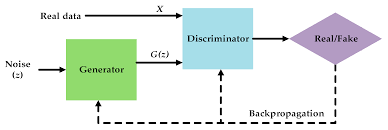
\includegraphics[width=0.6\textwidth]{images/gan_framework.png}
    \caption{GAN Framework}
    \label{fig:gan_framework}
\end{figure}

\paragraph{Discriminator Formulation.}

Assume there exists a generator $G$ as defined above. Let us assume we have a dataset $\mathcal{D}^\ast = \{x_1, ..., x_N\}$ which contains true data points, and a dataset $\mathcal{D} = \{x_1^{'}, ..., x_M^{'}\}$ containing generated data. We can define a distance function $D_{\phi}(x) \in [0, 1]$, to score whether a data point produced by the generator is similar to a data point from the true data. 

Now, since we have $\mathcal{D}^\ast$ and $\mathcal{D}$, we can learn such distance function by setting the following objective:
\begin{equation}
    \label{eq:gan_d}
    \max_{\phi} \Big\{ 
    \sum\limits_{x\sim\mathcal{D}^\ast} [D_{\phi}(x)] +
    \sum\limits_{x\sim\mathcal{D}} [1 - D_{\phi}(x)] \Big\}
\end{equation}
i.e., we want to maximize the distance function parametrized by $\phi$ such that the difference between discriminating against a true data point and a fake data point is as large as possible.

Note that we can also express the objective above as an expectation over samples \eqref{eq:gan_d_expect} and using base distributions $p$ and $q$ \eqref{eq:gan_d_base_distrib}:
\begin{equation}
    \label{eq:gan_d_expect}
    \max_{\phi} \Big\{ 
    \mathbb{E}_{D^\ast} [D_{\phi}(x)] + \mathbb{E}_\mathcal{D} [1 - D_{\phi}(x)] \Big\}
\end{equation}

\begin{equation}
    \label{eq:gan_d_base_distrib}
    \max_{\phi} \Big\{ 
    \sum\limits_{x\sim p(x)} [D_{\phi}(x)] +
    \sum\limits_{z\sim q(z)} [1 - D_{\phi}(G_{\theta}(z))] \Big\}
\end{equation}

\paragraph{Generator Formulation.}

Now, assume there exists a discriminator $D_{\phi}$ as formulated in the previous section. Our goal is to define a generator $G_\theta$ which is able to trick the discriminator. To do so, we want to learn its parameters $\theta$ following the objective below:
\begin{equation}
    \label{eq:gan_g}
    \min_{\theta} \Big\{ 
    \sum\limits_{z \sim p(z)} [1 - D_{\phi}(G_{\theta}(z))] \Big\} \\
\end{equation}

\paragraph{GAN Formulation.}

The GAN formulation combines both the generator objective and the discriminator objective together to learn both $G_\theta$ and $D_\phi$ simultaneously. It does so by setting the following min-max game:
\begin{align}
    \label{eq:gan}
    &\min_\theta \max_{\phi} \Big\{ 
    \sum\limits_{x\sim \mathcal{D}^\ast} [D_{\phi}(x)] +
    \sum\limits_{x\sim \mathcal{D}} [1 - D_{\phi}(x)] \Big\} \\
    &\min_\theta \max_{\phi} \Big\{ 
    \sum\limits_{x\sim \mathcal{D}^\ast} [\ln \{D_{\phi}(x)\}] +
    \sum\limits_{x\sim \mathcal{D}} [\ln\{1 - D_{\phi}(x)\}] \Big\} \quad \text{\footnotesize{"cross-entropy" formulation}}
\end{align}

If the distance function is differentiable, we can optimize for its parameters using gradient ascent with the following update equation:
\begin{equation}
    \phi = \phi + \mathbb{E}_{\mathcal{D}^\ast} [\nabla_\phi \ln \{D_{\phi}(x)\} ]
    + \mathbb{E}_{\mathcal{D}}[\nabla_\phi \ln\{1 - D_\phi(x)\}]
\end{equation}

Similarly, we can define the generator as a differentiable function and optimize it using gradient descent:
\begin{equation}
    \theta = \theta - \mathbb{E}_{\mathcal{D}}[\nabla_\theta \ln\{1 - D_\phi(x)\}]
\end{equation}

\paragraph{GAN Algorithm.}

Finally, the GAN algorithm is shown below:

\begin{algorithm}[H]
    \label{algo:gan}
    \caption{GAN}
    \begin{algorithmic}[1]
    \Function{GAN}{}
    \State $\mathcal{D}^\ast = \{ x_m\}_{m=1}^M \sim p^\ast (x)$  \hfill $\triangleright$ Obtain true data points from the distribution $p^\ast(x)$
    \For{$k=1, \dots K$}
    \State $\mathcal{D}_\theta = \{ x_n\}_{n=1}^N \sim G_\theta (z) | q(z)$ \hfill $\triangleright$ Obtain data points from the distribution $q(z)$ 
    \State $\phi = \phi + \mathbb{E}_{\mathcal{D}^\ast} [\nabla_\phi \ln \{D_{\phi}(x)\} ]
    + \mathbb{E}_{\mathcal{D}_\theta}[\nabla_\phi \ln\{1 - D_\phi(x)\}]$ \hfill $\triangleright$ Discriminator update 
    \State $\theta = \theta - \mathbb{E}_{\mathcal{D}_\theta}[\nabla_\theta \ln\{1 - D_\phi(x)\}]$ \hfill $\triangleright$ Generator update 
    \EndFor \\
    \Return $\boldsymbol{\theta}$
    \EndFunction
    \end{algorithmic}
\end{algorithm}

\subsection{Generative Adversarial Imitation Learning}

\subsubsection{Problem Setup}

GAIL \cite{ho2016gail} proposes a general framework for extracting a policy directly from data, as if it was obtained using RL followed by IRL. GAIL is formulated as a model-free imitation learning (IL) algorithm that exploits generative adversarial training to fit distributions of state-action pairs that define expert behavior. 

The GAIL framework defines a policy that is trying to generate trajectories similar to those produced by an expert. Then, it defines a scoring function which attempts to detect the generated trajectories. 

\subsubsection{Discriminator Formulation}

To formulate the GAIL discriminator, assume we are given a dataset containing expert trajectories $\mathcal{D}^\ast = \{s_1, a_1, \dots, s_N, a_N\}$, as well as fake trajectories $\mathcal{D}_\theta = \{s_1, a_1, \dots, s_M, a_M\}$. 

We want to learn a discriminator, $D_\phi (s, a) \in [0, 1]$, that is able to distinguish between a true state-action pair and generated one. This discriminator can framed as a cost function, where expert action induce low cost whereas fake actions induce a higher cost. 

Now, based on the objective derived in \eqref{eq:gan_d} we can formulate a slightly different optimization problem:
\begin{equation}
    \label{eq:gail_d}
    \max_{\phi} \Big\{ 
    \sum\limits_{s, a\sim\mathcal{D_\theta}} [D_{\phi}(s, a)] +
    \sum\limits_{s, a\sim\mathcal{D}^\ast} [1 - D_{\phi}(s, a)] \Big\}
\end{equation}
where instead of looking at a data point $x$ as before, we are looking at a state-action pair.  

\subsubsection{Generator Formulation}

The GAIL framework proposes a neural-based policy $G_\theta (s)$ that produces an action given a state. Note that this closely resembles the formulation of a generator network, except that instead of using noise as the input to the network, it uses a state. 

To generate a full trajectory, the policy is used auto-regressively along with an environment denoted by $\mathcal{E}$. The policy receives a state $s_{t}$ from the environment and uses it to produce an action $a_{t}$, s.t. $a_t = G_\theta (s_t)$. Then, the state-action pair is used as an input to the environment to produce the next state, $\mathcal{E}(s_t, a_t) \to s_{t+1}$. The new state becomes the current state of the policy and the process is repeated, thus, generating a trajectory of state-action pairs. 

Now, suppose we are given a cost function (discriminator) as formulated above. Thus, following the optimization problem in \eqref{eq:gan_g}, the GAIL objective for the generator can be expressed as:
\begin{equation}
    \label{eq:gail_g}
    \min_{\theta} \Big\{ 
    \sum\limits_{s,a \sim \mathcal{D}_\theta} [D_{\phi}(s, a)] \Big\} \\
\end{equation}

\subsubsection{GAIL Formulation}

As derived in Section~\ref{sec:gan}, we can combine the discriminator and generator objectives together to derive the GAIL min-max objective:
\begin{align}
    \label{eq:gail}
    &\min_\theta \max_{\phi} \Big\{ 
    \sum\limits_{s, a\sim \mathcal{D}_\theta} [\ln \{D_{\phi}(s, a)\}] +
    \sum\limits_{s, a\sim \mathcal{D}^\ast} [\ln\{1 - D_{\phi}(s, a)\}] \Big\}
\end{align}

\subsubsection{GAIL Algorithm}

Finally, the figure below shows a simplified version of the GAIL algorithm.

\begin{algorithm}[H]
    \label{algo:gail}
    \caption{Simplified GAIL}
    \begin{algorithmic}[1]
    \Function{GAIL}{}
    \State $\mathcal{D}^\ast = \{ \zeta^\ast_n\}_{m=1}^M$ where $\zeta_m^\ast = \{ s^{(0)}, a^{(0)}, \dots, s^{(T_m)} \} \sim \mathcal{E} | \pi^\ast$  
    \For{$k=1, \dots K$}
    \State $\mathcal{D}_\theta = \{ \zeta_n\}_{n=1}^N$ where $\zeta_n = \{s^{(0)}, a^{(0)}, \dots, s^{(T_n)} \} \sim \mathcal{E} | \pi_\theta$
    \State $\phi = \phi + \mathbb{E}_{\mathcal{D}_\theta} [\nabla_\phi \ln{D_\phi}(a, s)] + \mathbb{E}_{\mathcal{D}^\ast}[\nabla_\phi \ln \{1 - D_\phi(a, s)\}]$
    \State $\theta = \theta - \mathbb{E}_{\mathcal{D}_\theta}[\nabla_\theta \ln{\pi_\theta (a | s) Q(a, s)}]$
    \EndFor \\
    \Return $\boldsymbol{\theta}$
    \EndFunction
    \end{algorithmic}
\end{algorithm}

The algorithm above is similar to Algorithm~\ref{algo:gan}. The main difference lies in that the generator's optimization step in line 6 uses the policy gradient update which depends on $Q(s, a)$. 

The actual implementation in \cite{ho2016gail} follows the algorithm shown below. This version of the algorithm uses the Adam optimizer \cite{diederik2014adam} to update the discriminator parameters, which is depicted in line 5. Then, in line 6, the generator's update includes an additional term  which serves as a regularizer. Furthermore, the algorithm uses Trust Region Policy Optimization (TRPO) \cite{schulman2015trpo} to update the corresponding parameters.

\begin{algorithm}[H]
    \label{algo:gail_lambda}
    \caption{GAIL}
    \begin{algorithmic}[1]
    \Function{GAIL}{$\lambda$}
    \State $\mathcal{D}^\ast = \{ \zeta^\ast_n\}_{m=1}^M$ where $\zeta_m^\ast = \{ s^{(0)}, a^{(0)}, \dots, s^{(T_m)} \} \sim \mathcal{E} | \pi^\ast$ 
    \For{$k=1, \dots K$}
    \State $\mathcal{D}_\theta = \{ \zeta_n\}_{n=1}^N$ where $\zeta_n = \{s^{(0)}, a^{(0)}, \dots, s^{(T_n)} \} \sim \mathcal{E} | \pi_\theta$
    \State $\phi = $ \Call{ADAM}{$\mathbb{E}_{\mathcal{D}_\theta} [\nabla_\phi \ln{D_\phi}(a, s)] + \mathbb{E}_{\mathcal{D}^\ast}[\nabla_\phi \ln \{1 - D_\phi(a, s)\}]$}
    \State $\theta = $ \Call{TRPO}{$\mathbb{E}_{\mathcal{D}_\theta}[\nabla_\theta \ln{\pi_\theta (a | s) Q(a, s) - \lambda \nabla_\theta H(\pi_\theta)}]$}
    \EndFor \\
    \Return $\boldsymbol{\theta}$
    \EndFunction
    \end{algorithmic}
\end{algorithm}

\subsubsection{Theoretical Contributions}

Three main contributions that the GAIL paper made are:
\begin{enumerate}
    \item Unifies IRL with the following objective:
    \begin{equation}
        IRL_\psi(\pi^\ast) = \max\limits_c \min\limits_\pi (-H(\pi) 
        + \mathbb{E}_\pi [\sum\limits_{t=0}^\infty \gamma^t c(s, a)]) 
        - \mathbb{E}_{\pi^\ast}[\sum\limits_{t=0}^\infty \gamma^t c(s, a)] - \psi(c),
    \end{equation}
    where the terms represent the maximum causal entropy, the expert policy cost and the regularizer, respectively. 
    \item Shows that the choice of regularizer leads to different types of IRL
    \item GAIL's regularizer is given by:
    \begin{align}
    \psi_{GAIL}(c) = \left\{ \begin{array}{cc} 
               \mathbb{E}_{\pi^\ast}[-c(s, a) - \ln\{ 1 - e^{c(s, a)}\}] & \hspace{5mm} \text{if } c(s, a)\leq 0 \\
                +\infty & \hspace{5mm} \text{ otherwise }
                \end{array} \right.
    \end{align}
\end{enumerate}

%\section*{References}
%Include your references here. Please cite any resources you found useful.	
%Populate the refs.bib file or list your references manually. Be consistent in formatting!
{
\bibliography{refs}
\bibliographystyle{unsrt}
}


%This section provides any relevant background material that was not covered in the lectures, but was found to be useful for understanding the material. 
%For example, derivations, theory underlying techniques employed, etc. 

%Additionally, this section can summarizes applications or extensions of these techniques found in the literature. 

\end{document} % Done!


